\documentclass{standalone}
\usepackage{tikz}
\usetikzlibrary{patterns, positioning}


\begin{document}
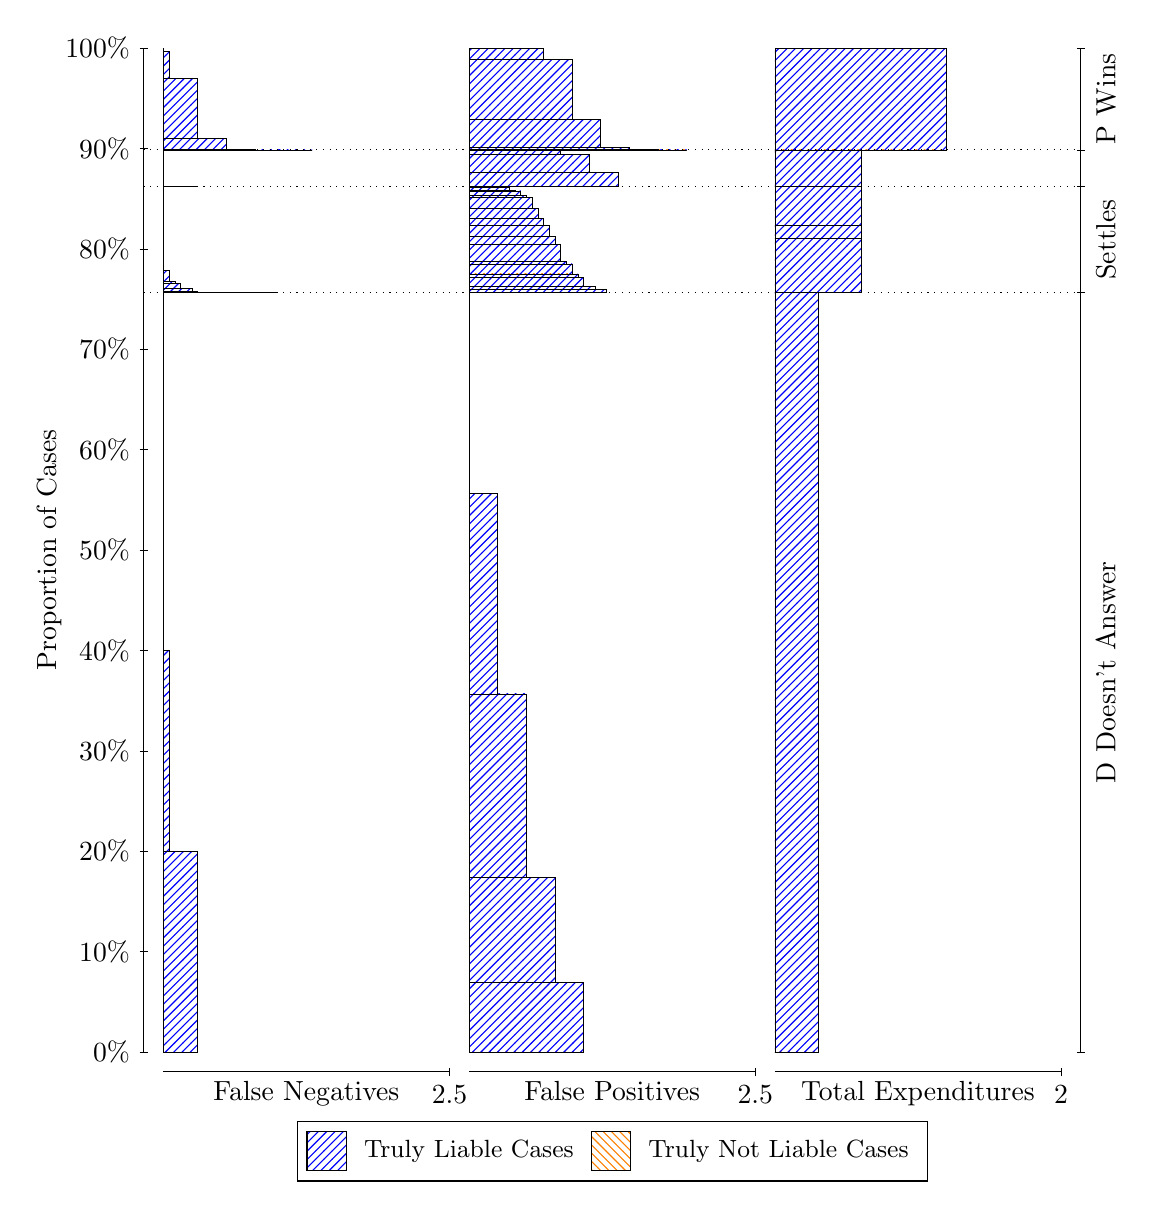
\begin{tikzpicture}
\draw[black, very thin] (1.5,1.75) -- (1.5,14.5);
\node[rotate=90, text=black, anchor=center] at (0.3, 8.125) {Proportion of Cases};
\draw[black, very thin] (1.45,1.75) -- (1.55,1.75);
\node[text=black, anchor=east] at (1.45, 1.75) {0\%};
\draw[black, very thin] (1.45,3.025) -- (1.55,3.025);
\node[text=black, anchor=east] at (1.45, 3.025) {10\%};
\draw[black, very thin] (1.45,4.3) -- (1.55,4.3);
\node[text=black, anchor=east] at (1.45, 4.3) {20\%};
\draw[black, very thin] (1.45,5.575) -- (1.55,5.575);
\node[text=black, anchor=east] at (1.45, 5.575) {30\%};
\draw[black, very thin] (1.45,6.85) -- (1.55,6.85);
\node[text=black, anchor=east] at (1.45, 6.85) {40\%};
\draw[black, very thin] (1.45,8.125) -- (1.55,8.125);
\node[text=black, anchor=east] at (1.45, 8.125) {50\%};
\draw[black, very thin] (1.45,9.4) -- (1.55,9.4);
\node[text=black, anchor=east] at (1.45, 9.4) {60\%};
\draw[black, very thin] (1.45,10.675) -- (1.55,10.675);
\node[text=black, anchor=east] at (1.45, 10.675) {70\%};
\draw[black, very thin] (1.45,11.95) -- (1.55,11.95);
\node[text=black, anchor=east] at (1.45, 11.95) {80\%};
\draw[black, very thin] (1.45,13.225) -- (1.55,13.225);
\node[text=black, anchor=east] at (1.45, 13.225) {90\%};
\draw[black, very thin] (1.45,14.5) -- (1.55,14.5);
\node[text=black, anchor=east] at (1.45, 14.5) {100\%};

\draw[black, very thin] (13.4,1.75) -- (13.4,14.5);
\draw[black, very thin] (13.35,1.75) -- (13.45,1.75);
\node[anchor=west] at (13.35, 1.75) {};
\draw[black, very thin] (13.35,11.395) -- (13.45,11.395);
\node[anchor=west] at (13.35, 11.395) {};
\draw[black, very thin] (13.35,12.745) -- (13.45,12.745);
\node[anchor=west] at (13.35, 12.745) {};
\draw[black, very thin] (13.35,13.207) -- (13.45,13.207);
\node[anchor=west] at (13.35, 13.207) {};
\draw[black, very thin] (13.35,14.5) -- (13.45,14.5);
\node[anchor=west] at (13.35, 14.5) {};

\draw[black, very thin, pattern color=blue, pattern=north east lines] (1.75,1.75) rectangle (2.186,4.2999);
\draw[black, very thin, pattern color=blue, pattern=north east lines] (1.75,4.2999) rectangle (1.8227,6.8481);
\draw[black, very thin, pattern color=orange, pattern=north west lines] (1.75,6.8481) rectangle (1.75,6.8481);
\draw[black, very thin, pattern color=blue, pattern=north east lines] (1.75,6.8481) rectangle (1.75,11.395);
\draw[black, very thin, pattern color=blue, pattern=north east lines] (1.75,11.395) rectangle (3.2033,11.395);
\draw[black, very thin, pattern color=blue, pattern=north east lines] (1.75,11.395) rectangle (3.058,11.395);
\draw[black, very thin, pattern color=blue, pattern=north east lines] (1.75,11.395) rectangle (2.9127,11.395);
\draw[black, very thin, pattern color=blue, pattern=north east lines] (1.75,11.395) rectangle (2.84,11.395);
\draw[black, very thin, pattern color=blue, pattern=north east lines] (1.75,11.395) rectangle (2.7673,11.395);
\draw[black, very thin, pattern color=blue, pattern=north east lines] (1.75,11.395) rectangle (2.6947,11.395);
\draw[black, very thin, pattern color=blue, pattern=north east lines] (1.75,11.395) rectangle (2.622,11.395);
\draw[black, very thin, pattern color=blue, pattern=north east lines] (1.75,11.395) rectangle (2.5493,11.395);
\draw[black, very thin, pattern color=blue, pattern=north east lines] (1.75,11.395) rectangle (2.4767,11.396);
\draw[black, very thin, pattern color=blue, pattern=north east lines] (1.75,11.396) rectangle (2.404,11.396);
\draw[black, very thin, pattern color=blue, pattern=north east lines] (1.75,11.396) rectangle (2.3313,11.398);
\draw[black, very thin, pattern color=blue, pattern=north east lines] (1.75,11.398) rectangle (2.3313,11.398);
\draw[black, very thin, pattern color=blue, pattern=north east lines] (1.75,11.398) rectangle (2.2587,11.398);
\draw[black, very thin, pattern color=blue, pattern=north east lines] (1.75,11.398) rectangle (2.186,11.408);
\draw[black, very thin, pattern color=blue, pattern=north east lines] (1.75,11.408) rectangle (2.1133,11.446);
\draw[black, very thin, pattern color=blue, pattern=north east lines] (1.75,11.446) rectangle (2.0407,11.452);
\draw[black, very thin, pattern color=blue, pattern=north east lines] (1.75,11.452) rectangle (1.968,11.512);
\draw[black, very thin, pattern color=blue, pattern=north east lines] (1.75,11.512) rectangle (1.968,11.512);
\draw[black, very thin, pattern color=blue, pattern=north east lines] (1.75,11.512) rectangle (1.8953,11.533);
\draw[black, very thin, pattern color=blue, pattern=north east lines] (1.75,11.533) rectangle (1.8227,11.677);
\draw[black, very thin, pattern color=orange, pattern=north west lines] (1.75,11.677) rectangle (1.75,11.677);
\draw[black, very thin, pattern color=blue, pattern=north east lines] (1.75,11.677) rectangle (1.75,12.745);
\draw[black, very thin, pattern color=blue, pattern=north east lines] (1.75,12.745) rectangle (2.186,12.745);
\draw[black, very thin, pattern color=blue, pattern=north east lines] (1.75,12.745) rectangle (1.8227,12.745);
\draw[black, very thin, pattern color=orange, pattern=north west lines] (1.75,12.745) rectangle (1.75,12.745);
\draw[black, very thin, pattern color=blue, pattern=north east lines] (1.75,12.745) rectangle (1.75,13.207);
\draw[black, very thin, pattern color=blue, pattern=north east lines] (1.75,13.207) rectangle (3.6393,13.207);
\draw[black, very thin, pattern color=blue, pattern=north east lines] (1.75,13.207) rectangle (3.276,13.207);
\draw[black, very thin, pattern color=blue, pattern=north east lines] (1.75,13.207) rectangle (2.9127,13.21);
\draw[black, very thin, pattern color=blue, pattern=north east lines] (1.75,13.21) rectangle (2.5493,13.348);
\draw[black, very thin, pattern color=blue, pattern=north east lines] (1.75,13.348) rectangle (2.186,13.348);
\draw[black, very thin, pattern color=blue, pattern=north east lines] (1.75,13.348) rectangle (2.186,14.111);
\draw[black, very thin, pattern color=blue, pattern=north east lines] (1.75,14.111) rectangle (1.8227,14.111);
\draw[black, very thin, pattern color=blue, pattern=north east lines] (1.75,14.111) rectangle (1.8227,14.465);
\draw[black, very thin, pattern color=orange, pattern=north west lines] (1.75,14.465) rectangle (1.75,14.465);
\draw[black, very thin, pattern color=blue, pattern=north east lines] (1.75,14.465) rectangle (1.75,14.5);
\draw[black, very thin, pattern color=orange, pattern=north west lines] (5.6333,1.75) rectangle (7.0867,1.75);
\draw[black, very thin, pattern color=blue, pattern=north east lines] (5.6333,1.75) rectangle (7.0867,2.6385);
\draw[black, very thin, pattern color=blue, pattern=north east lines] (5.6333,2.6385) rectangle (6.7233,3.9673);
\draw[black, very thin, pattern color=blue, pattern=north east lines] (5.6333,3.9673) rectangle (6.36,6.2966);
\draw[black, very thin, pattern color=blue, pattern=north east lines] (5.6333,6.2966) rectangle (5.9967,8.8447);
\draw[black, very thin, pattern color=blue, pattern=north east lines] (5.6333,8.8447) rectangle (5.6333,11.395);
\draw[black, very thin, pattern color=orange, pattern=north west lines] (5.6333,11.395) rectangle (7.3773,11.395);
\draw[black, very thin, pattern color=blue, pattern=north east lines] (5.6333,11.395) rectangle (7.3773,11.437);
\draw[black, very thin, pattern color=orange, pattern=north west lines] (5.6333,11.437) rectangle (7.232,11.437);
\draw[black, very thin, pattern color=blue, pattern=north east lines] (5.6333,11.437) rectangle (7.232,11.474);
\draw[black, very thin, pattern color=orange, pattern=north west lines] (5.6333,11.474) rectangle (7.0867,11.474);
\draw[black, very thin, pattern color=blue, pattern=north east lines] (5.6333,11.474) rectangle (7.0867,11.591);
\draw[black, very thin, pattern color=blue, pattern=north east lines] (5.6333,11.591) rectangle (7.014,11.633);
\draw[black, very thin, pattern color=orange, pattern=north west lines] (5.6333,11.633) rectangle (6.9413,11.633);
\draw[black, very thin, pattern color=blue, pattern=north east lines] (5.6333,11.633) rectangle (6.9413,11.758);
\draw[black, very thin, pattern color=blue, pattern=north east lines] (5.6333,11.758) rectangle (6.8687,11.792);
\draw[black, very thin, pattern color=orange, pattern=north west lines] (5.6333,11.792) rectangle (6.796,11.792);
\draw[black, very thin, pattern color=blue, pattern=north east lines] (5.6333,11.792) rectangle (6.796,12.007);
\draw[black, very thin, pattern color=blue, pattern=north east lines] (5.6333,12.007) rectangle (6.7233,12.111);
\draw[black, very thin, pattern color=orange, pattern=north west lines] (5.6333,12.111) rectangle (6.6507,12.111);
\draw[black, very thin, pattern color=blue, pattern=north east lines] (5.6333,12.111) rectangle (6.6507,12.248);
\draw[black, very thin, pattern color=blue, pattern=north east lines] (5.6333,12.248) rectangle (6.578,12.333);
\draw[black, very thin, pattern color=blue, pattern=north east lines] (5.6333,12.333) rectangle (6.5053,12.341);
\draw[black, very thin, pattern color=orange, pattern=north west lines] (5.6333,12.341) rectangle (6.5053,12.341);
\draw[black, very thin, pattern color=blue, pattern=north east lines] (5.6333,12.341) rectangle (6.5053,12.463);
\draw[black, very thin, pattern color=blue, pattern=north east lines] (5.6333,12.463) rectangle (6.4327,12.607);
\draw[black, very thin, pattern color=blue, pattern=north east lines] (5.6333,12.607) rectangle (6.36,12.627);
\draw[black, very thin, pattern color=blue, pattern=north east lines] (5.6333,12.627) rectangle (6.2873,12.687);
\draw[black, very thin, pattern color=blue, pattern=north east lines] (5.6333,12.687) rectangle (6.2147,12.694);
\draw[black, very thin, pattern color=blue, pattern=north east lines] (5.6333,12.694) rectangle (6.142,12.694);
\draw[black, very thin, pattern color=blue, pattern=north east lines] (5.6333,12.694) rectangle (6.142,12.732);
\draw[black, very thin, pattern color=blue, pattern=north east lines] (5.6333,12.732) rectangle (6.0693,12.742);
\draw[black, very thin, pattern color=blue, pattern=north east lines] (5.6333,12.742) rectangle (5.9967,12.742);
\draw[black, very thin, pattern color=blue, pattern=north east lines] (5.6333,12.742) rectangle (5.924,12.744);
\draw[black, very thin, pattern color=blue, pattern=north east lines] (5.6333,12.744) rectangle (5.8513,12.744);
\draw[black, very thin, pattern color=blue, pattern=north east lines] (5.6333,12.744) rectangle (5.7787,12.744);
\draw[black, very thin, pattern color=blue, pattern=north east lines] (5.6333,12.744) rectangle (5.7787,12.745);
\draw[black, very thin, pattern color=blue, pattern=north east lines] (5.6333,12.745) rectangle (5.706,12.745);
\draw[black, very thin, pattern color=blue, pattern=north east lines] (5.6333,12.745) rectangle (5.6333,12.745);
\draw[black, very thin, pattern color=orange, pattern=north west lines] (5.6333,12.745) rectangle (7.5227,12.745);
\draw[black, very thin, pattern color=blue, pattern=north east lines] (5.6333,12.745) rectangle (7.5227,12.919);
\draw[black, very thin, pattern color=blue, pattern=north east lines] (5.6333,12.919) rectangle (7.1593,13.147);
\draw[black, very thin, pattern color=blue, pattern=north east lines] (5.6333,13.147) rectangle (6.796,13.207);
\draw[black, very thin, pattern color=blue, pattern=north east lines] (5.6333,13.207) rectangle (6.4327,13.207);
\draw[black, very thin, pattern color=blue, pattern=north east lines] (5.6333,13.207) rectangle (6.0693,13.207);
\draw[black, very thin, pattern color=orange, pattern=north west lines] (5.6333,13.207) rectangle (8.3947,13.207);
\draw[black, very thin, pattern color=blue, pattern=north east lines] (5.6333,13.207) rectangle (8.3947,13.207);
\draw[black, very thin, pattern color=orange, pattern=north west lines] (5.6333,13.207) rectangle (8.0313,13.207);
\draw[black, very thin, pattern color=blue, pattern=north east lines] (5.6333,13.207) rectangle (8.0313,13.208);
\draw[black, very thin, pattern color=orange, pattern=north west lines] (5.6333,13.208) rectangle (7.668,13.208);
\draw[black, very thin, pattern color=blue, pattern=north east lines] (5.6333,13.208) rectangle (7.668,13.242);
\draw[black, very thin, pattern color=orange, pattern=north west lines] (5.6333,13.242) rectangle (7.3047,13.242);
\draw[black, very thin, pattern color=blue, pattern=north east lines] (5.6333,13.242) rectangle (7.3047,13.597);
\draw[black, very thin, pattern color=orange, pattern=north west lines] (5.6333,13.597) rectangle (6.9413,13.597);
\draw[black, very thin, pattern color=blue, pattern=north east lines] (5.6333,13.597) rectangle (6.9413,14.36);
\draw[black, very thin, pattern color=blue, pattern=north east lines] (5.6333,14.36) rectangle (6.578,14.498);
\draw[black, very thin, pattern color=blue, pattern=north east lines] (5.6333,14.498) rectangle (6.2147,14.5);
\draw[black, very thin, pattern color=blue, pattern=north east lines] (5.6333,14.5) rectangle (5.8513,14.5);
\draw[black, very thin, pattern color=blue, pattern=north east lines] (5.6333,14.5) rectangle (5.6333,14.5);
\draw[black, very thin, pattern color=orange, pattern=north west lines] (9.5167,1.75) rectangle (10.062,1.75);
\draw[black, very thin, pattern color=blue, pattern=north east lines] (9.5167,1.75) rectangle (10.062,11.395);
\draw[black, very thin, pattern color=orange, pattern=north west lines] (9.5167,11.395) rectangle (10.607,11.395);
\draw[black, very thin, pattern color=blue, pattern=north east lines] (9.5167,11.395) rectangle (10.607,12.084);
\draw[black, very thin, pattern color=orange, pattern=north west lines] (9.5167,12.084) rectangle (10.607,12.084);
\draw[black, very thin, pattern color=blue, pattern=north east lines] (9.5167,12.084) rectangle (10.607,12.245);
\draw[black, very thin, pattern color=orange, pattern=north west lines] (9.5167,12.245) rectangle (10.607,12.245);
\draw[black, very thin, pattern color=blue, pattern=north east lines] (9.5167,12.245) rectangle (10.607,12.745);
\draw[black, very thin, pattern color=orange, pattern=north west lines] (9.5167,12.745) rectangle (10.607,12.745);
\draw[black, very thin, pattern color=blue, pattern=north east lines] (9.5167,12.745) rectangle (10.607,13.207);
\draw[black, very thin, pattern color=orange, pattern=north west lines] (9.5167,13.207) rectangle (11.697,13.207);
\draw[black, very thin, pattern color=blue, pattern=north east lines] (9.5167,13.207) rectangle (11.697,14.5);
\draw[black, dotted] (1.5,11.395) -- (13.4,11.395);
\draw[black, dotted] (1.5,12.745) -- (13.4,12.745);
\draw[black, dotted] (1.5,13.207) -- (13.4,13.207);
\draw[black, very thin] (1.75,1.5) -- (5.3833,1.5);
\node[text=black, anchor=north] at (3.5667, 1.5) {False Negatives};
\draw[black, very thin] (5.3833,1.45) -- (5.3833,1.55);
\node[text=black, anchor=north] at (5.3833, 1.45) {2.5};

\draw[black, very thin] (5.6333,1.5) -- (9.2667,1.5);
\node[text=black, anchor=north] at (7.45, 1.5) {False Positives};
\draw[black, very thin] (9.2667,1.45) -- (9.2667,1.55);
\node[text=black, anchor=north] at (9.2667, 1.45) {2.5};

\draw[black, very thin] (9.5167,1.5) -- (13.15,1.5);
\node[text=black, anchor=north] at (11.333, 1.5) {Total Expenditures};
\draw[black, very thin] (13.15,1.45) -- (13.15,1.55);
\node[text=black, anchor=north] at (13.15, 1.45) {2};

\node[text=black, centered, rotate=90] at (13.72, 6.5723) {D Doesn't Answer};
\node[text=black, centered, rotate=90] at (13.72, 12.07) {Settles};

\node[text=black, centered, rotate=90] at (13.72, 13.854) {P Wins};

\draw (7.449999999999999,1.5) node[draw=none] (baseCoordinate) {};
\begin{scope}[align=center]
        \matrix[scale=0.5, draw=black, below=0.5cm of baseCoordinate, nodes={draw}, column sep=0.1cm]{
            \node[rectangle, draw, minimum width=0.5cm, minimum height=0.5cm, pattern color=blue, pattern=north east lines] {}; &
            \node[draw=none, font=\small, text=black] (B) {Truly Liable Cases}; &
            \node[rectangle, draw, minimum width=0.5cm, minimum height=0.5cm, pattern color=orange, pattern=north west lines] {}; &
            \node[draw=none, font=\small, text=black] (B) {Truly Not Liable Cases}; \\
            };
\end{scope}

\end{tikzpicture}
\end{document}